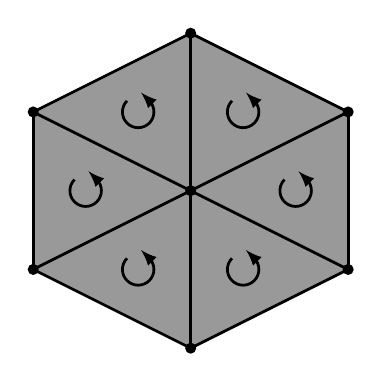
\begin{tikzpicture}[>=latex, line width=1pt]
  % Coords
  \coordinate (V0) at (2,0);
  \coordinate (V1) at (2,2);
  \coordinate (V2) at (0,1);
  \coordinate (V3) at (4,1);
  \coordinate (V4) at (4,-1);
  \coordinate (V5) at (0,-1);
 \coordinate (V6) at (2,-2);

\fill[opacity=0.4]  (V1) -- (V3) -- (V4) -- (V6) -- (V5) -- (V2);
  % Arrows\tilde{\sigma}
  \draw(V0) -- (V1);
  \draw(V1) --  (V2);
  \draw(V0) -- (V2);
  \draw(V1) --  (V3);
  \draw(V0) -- (V3);
   \draw(V0) -- (V4);
  \draw(V0) -- (V5);
  \draw(V5) --  (V2);
  \draw(V3) --  (V4);
 \draw(V4) -- (V6);
\draw(V0) -- (V6);
\draw(V6) -- (V5);
  % Points
  \fill[] (V0) circle (2pt);
  \fill[] (V1) circle (2pt);
  \fill[] (V2) circle (2pt);
  \fill[] (V3) circle (2pt);
  \fill[] (V4) circle (2pt);
  \fill[] (V5)circle (2pt);
 \fill[] (V6)circle (2pt);



%circumcenter
\coordinate (CC1) at (1.333,1);
\coordinate (CC0) at (2.666,1);
\coordinate (CC3) at (1.333,-1);
\coordinate (CC2) at (0.666,0);
\coordinate (CC4) at (2.666,-1);
\coordinate (CC5) at (3.333,0);

\draw[->] (CC0) + (135:0.2) arc (135:405:0.2) --++ (-3pt,3pt);
\draw[->] (CC1) + (135:0.2) arc (135:405:0.2) --++ (-3pt,3pt);
\draw[->] (CC2) + (135:0.2) arc (135:405:0.2) --++ (-3pt,3pt);
\draw[->] (CC3) + (135:0.2) arc (135:405:0.2) --++ (-3pt,3pt);
\draw[->] (CC4) + (135:0.2) arc (135:405:0.2) --++ (-3pt,3pt);
\draw[->] (CC5) + (135:0.2) arc (135:405:0.2) --++ (-3pt,3pt);
%\fill[red] (CC0) circle (2pt);
%\fill[red] (CC1) circle (2pt);
%\fill[red] (CC2) circle (2pt);
%\fill[red] (CC3) circle (2pt);
%\fill[red] (CC4) circle (2pt);
%\fill[red] (CC5) circle (2pt);


%\coordinate (C01) at (2,1);
%\coordinate (C02) at (1,0.5);
%\coordinate (C03) at (3,0.5);
%\coordinate (C05) at (1,-0.5);
%\coordinate (C04) at (3,-0.5);
%\coordinate (C06) at (2,-1);

% \fill[red] (C01) circle (2pt);
%\fill[red] (C02) circle (2pt);
%\fill[red] (C03) circle (2pt);
%\fill[red] (C05) circle (2pt);
%\fill[red] (C04) circle (2pt);
%\fill[red] (C06) circle (2pt);

%\coordinate (C12) at (1,1.5);
%\coordinate (C25) at (0,0);
%\coordinate (C56) at (1,-1.5);
%\coordinate (C46) at (3,-1.5);
%\coordinate (C34) at (4,0);
%\coordinate (C13) at (3,1.5);

%\fill[red] (C12) circle (2pt);
%\fill[red] (C25) circle (2pt);
%\fill[red] (C56) circle (2pt);
%\fill[red] (C46) circle (2pt);
%\fill[red] (C34) circle (2pt);
%\fill[red] (C13) circle (2pt);
  %\draw[line width=1pt, ->,style=dotted] (CC0) -- (CC1);
  %\draw[line width=1pt, ->,style=dotted] (CC1) -- (CC2);
 % \draw[line width=1pt, ->,style=dotted] (CCm) -- (CC0);
 % \draw[line width=1pt,style=dotted] (CC2) -- (CCC3);
 % \draw[line width=1pt,->,style=dotted] (CCC4) -- (CCm);

\end{tikzpicture}

